%++++++++++++++++++++++++++++++++++++++++
% Don't modify this section unless you know what you're doing!
\documentclass[letterpaper,12pt]{article}
\usepackage[utf8]{inputenc}
\usepackage{float}
\usepackage{tabularx} % extra features for tabular environment
\usepackage{amsmath}  % improve math presentation
\usepackage{graphicx} % takes care of graphic including machinery
\usepackage[margin=1in,letterpaper]{geometry} % decreases margins
\usepackage{cite} % takes care of citations
\usepackage[final]{hyperref} % adds hyper links inside the generated pdf file
\usepackage[table,xcdraw]{xcolor}
\hypersetup{
	colorlinks=true,       % false: boxed links; true: colored links
	linkcolor=blue,        % color of internal links
	citecolor=blue,        % color of links to bibliography
	filecolor=magenta,     % color of file links
	urlcolor=blue         
}
%++++++++++++++++++++++++++++++++++++++++


\begin{document}

\title{Práctica 3 - Ruteo}
\author{Matthew Aguerreberry, Natasha Tomattis}
\date{\today}
\maketitle

% \begin{abstract} 
% \end{abstract}


\section{Practica de Ruteo - OSPF}
	\begin{figure}[ht] 
			
		\centering 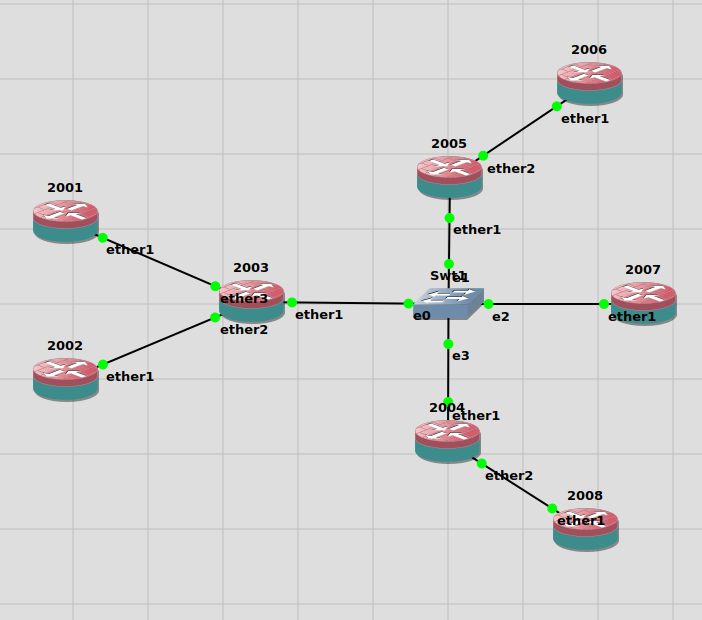
\includegraphics[width=0.8\columnwidth]{figure/topo_figura1.png}
		\caption{
				\label{fig:samplesetup} % spaces are big no-no 
				Implementación Ejercicio 1.
		}
	\end{figure}
	\begin{enumerate}
		\item \textbf{Conectar los routers, switchs y nodos según el diagrama de la figura 1.}
		\item \textbf{Configurar interfaces de acuerdo al diagrama.}
		\item \textbf{¿Configurar OSPF en todas los routers respetando las áreas según el diagrama. Es posible alcanzar todas las redes?} \\
		Si, todas las redes son compartidas a través de OSPF.
		\item \textbf{Los routers de las áreas no backbone, conocen todas las rutas a las demás redes?}\\
		Si, la división de áreas no limita la propagación de rutas OSPF. Solo limita el alcance de algunos mensajes LSA.
		\item \textbf{Observando el área backbone, que router fue elegido como DR y cual como BDR? ¿Por qué fueron elegidos esos routers?}\\
		Se eligió el router con el router ID más alto de la red 10.0.10.0/24 como DR y el subsiguiente como BDR. El router ID, por defecto en mikrotik, toma el valor de IP más bajo de las interfaces activas del dispositivo.
		\item \textbf{Elegir uno de los routers que no cumple una de esas funciones y configurarlo para que sea DR (no debe modificar el direccionamiento) ¿De qué manera/s puede hacer esto? Seleccione una para lograr lo solicitado.}\\
		Esto se puede lograr de varias maneras, por un lado se puede cambiar la prioridad del router la cual sera utilizada a la hora de la elección del DR; por otro lado se puede modificar el router ID ya sea a través de la configuración explicita de este parámetro o la configuración de una interfaz loopback con una dirección de mayor valar que los otros router ID. En nuestro caso configuramos una interfaz loopback1 en el dispositivo 2003 para que esta sea utilizada como router ID, como se puede ver en la imagen a continuación.
		\begin{figure}[H] 
			
			\centering 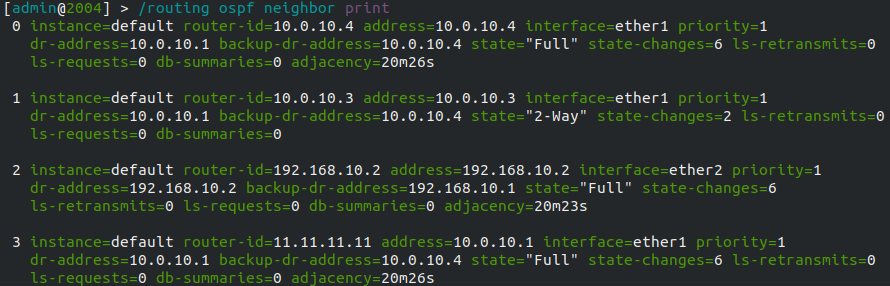
\includegraphics[width=0.5\columnwidth]{figure/int_loopback.png}
			\caption{
					\label{fig:samplesetup} % spaces are big no-no 
					Configuración de la interfaz loopback en el router 2003.
			}
		\end{figure} 
		\begin{figure}[H] 
			
			\centering 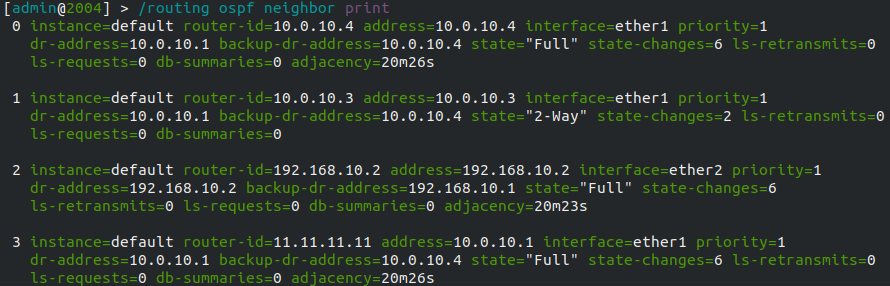
\includegraphics[width=0.8\columnwidth]{figure/new_dr.png}
			\caption{
					\label{fig:samplesetup} % spaces are big no-no 
					Selección de la IP configurada en loopback como router ID. Elección de nuevo DR.
			}
		\end{figure}
		\item \textbf{¿Por qué se recomienda definir una dirección de loopback cuando se utiliza OSPF?}\\
		Para poder controlar la selección del router ID, y por consiguiente la selección del router designado. Ya que si no se configura una interfaz loopback, esta decisión depende de las interfaces configuradas, las cuales pueden cambiar dinámicamente. De este modo, el administrador podría seleccionar un equipo con mejores características para ser siempre DR.
		\item \textbf{Explique los distintos tipos de áreas en OSPF}
		\begin{itemize}
			\item \textbf{stub área} Evita que entren LSA tipo 5 al área, esto quiere decir que rutas externas a OSPF no serán compartidas dentro del área. En lugar de advertir estas rutas internamente, el ABR(Area Border Router) crea un default gateway a través de si mismo. Asi, todos los paquetes destinados a las rutas externas serán enviados a través del ABR
			\item \textbf{totally stubby área} Actúa del mismo modo que \textit{stub área}, pero evitando que LSA tipo 3 entren al área, en este caso las rutas que no serán advertidas internamente serán las \textit{summary área}. De este modo, el área solo conocerá de sus propias rutas, los paquetes dirigidos a otras a áreas o a rutas externas serán enviados a través del ABR que se comporta como default gateway. 
			\item \textbf{NSSA} 
		\end{itemize}
		\item \textbf{En las áreas no backbone, ¿tambiénse elige un DR y un BDR?}\\
		Sí.
		\item \textbf{Definir el área 10 como área stub. ¿Qué sucede con la tabla de ruteo en el router 2001?}\\
		Se le agrega un default gateway, ya que establecer un área stub impide que el área conozca de rutas externas a OSPF, ete permite el acceso a rutas externas si las hubiera a través de 2003(ABR). En este caso como todas las rutas aprendidas son por OSPF, no se eliminan entradas en la tabla.
		\begin{figure}[H] 
			
			\centering 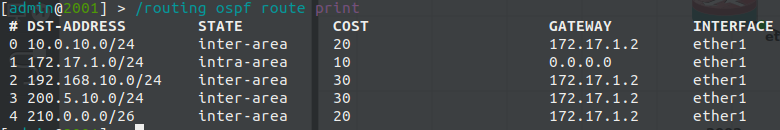
\includegraphics[width=0.7\columnwidth]{figure/routes_default_area.png}
			\caption{
					\label{fig:samplesetup} % spaces are big no-no 
					Rutas en 2001 antes de la configuración como stub área.
			}
		\end{figure} 
		\begin{figure}[H] 
			
			\centering 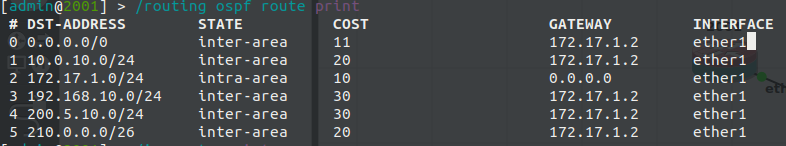
\includegraphics[width=0.7\columnwidth]{figure/routes_stub_area.png}
			\caption{
					\label{fig:samplesetup} % spaces are big no-no 
					Rutas en 2001 después de la configuración como stub área.
			}
		\end{figure}
		\item \textbf{¿Cómo definiría el área 10 para que 2001 solo aprenda de 2003 una ruta default?}\\
		Esto se puede lograr configurando el área 10 como \textit{totally stubby área}, este tipo de configuración impide que se intercambien LSAs de tipo 3 que contienen información sobre las rutas de las otras áreas. El comando utilizado en este caso fue \textit{"/routing ospf área set numbers=1 type=stub inject-summary-lsa=no"}
		\begin{figure}[H] 
			
			\centering 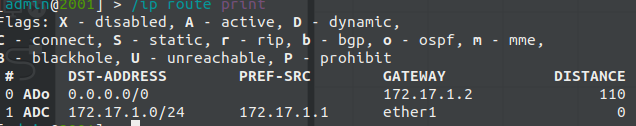
\includegraphics[width=0.7\columnwidth]{figure/routes_totally_stub.png}
			\caption{
					\label{fig:samplesetup} % spaces are big no-no 
					Rutas en 2001 después de la configuración como totally stubby área.
			}
		\end{figure}
		\item \textbf{Seleccionar un router que no sea DR ni BDR y deshabilitar la interface que se conecta contra el área no backbone (por ej. si selecciona el router 2004 deshabilitar la interface ether2). Antes de hacer esto habilitar la captura de paquetes en uno de los enlaces del backbone)}
		
		\item \textbf{¿Qué mensaje envía el router seleccionado en el área backbone? ¿A quién se lo envía? ¿Qué dirección utiliza? ¿Qué hace el receptor de este mensaje?}\\
		El router envía un mensaje LSA Update, con un LSA de tipo 1 (Router Update) a la dirección multicast 224.0.0.6 (Grupo conformado por DR y BDR). El DR envía el mismo mensaje a la dirección multicast 224.0.0.5 (Grupo conformado por todos los routers), para que actualicen sus bases de datos.
		\begin{figure}[H] 
			
			\centering 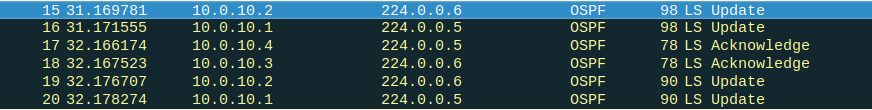
\includegraphics[width=0.7\columnwidth]{figure/2004_ether2_down.png}
			\caption{
					\label{fig:samplesetup} % spaces are big no-no 
					Mensajes en el área backbone luego de deshabilitar una interfaz.
			}
		\end{figure}
		\item \textbf{¿Cómo calcula OSPF el mejor camino a una red? ¿Qué algoritmo utiliza?}\\
		El cálculo del mejor camino es en base al ancho de banda de los enlaces, utilizando el algoritmo de Dijkstra.

		\item \textbf{Agregar un nuevo router a la topología según la figura 2}

		\item \textbf{Habilitar OSPF en el nuevo router y enlace agregado}
		
		\item \textbf{En el router 2009, agregar una red loopback, lo0=2.2.2.2/24, y publicarla por OSPF.}
		
		\item \textbf{¿Qué sucede con la tabla de ruteo del router 2002 una vez que se habilita OSPF en la interface ether2? Y 2009, ¿aprende algo por OSPF?}\\
		El router 2002 aprende las rutas del área 169 publicadas por 2009, es decir, las redes 169.192.30.64/28 y 2.2.2.0/24. Por su parte, 2009 aprende las rutas del área 200.
		
		\item \textbf{¿Es posible solucionar esto para que las redes del área 169 sean accesibles desde el resto del dominio OSPF?}\\
		Si, empleando enlaces virtuales que permiten comunicar dos áreas no adyacentes a través de un área de tránsito. Este tipo de áreas necesita dos routers ABRs para pasar tráfico desde un área a otra.\\
		Entonces, el área 200 será de tránsito para comunicar el área 169 con la backbone y de esta manera las redes del área 169 serán accesibles desde el resto del dominio OSPF.
		
		\item \textbf{Agregar un nuevo router a la topologia según la figura 3}

		\item \textbf{Configurar el nuevo enlace y router con RIPv2}
		
		\item \textbf{En el router 2010, agregar una red loopback, lo0=220.0.20.1/24, y publicarla por RIPv2.}
		
		\item \textbf{¿Qué debería hacer el router 2007 para que el dominio OSPF aprenda la red configurada en el paso anterior? ¿Cómo se conocería a ese router en la terminología de OSPF? (Hint.: investigue el concepto de redistribución)}\\
		En la terminología de OSPF el router 2007 sería conocido como Autonomous System Border Router (ASBR), debido a que se encuentra en la frontera del sistema autonomo administrado por OSPF y a su vez se conecta con otro sistema autónomo en este caso, administrado por RIP. Para que OSPF aprenda las rutas que administra RIP, es necesario aplicar redistribución. De esta forma, 2007 va a advertir a OSPF de las rutas aprendidas por RIP. \\
		Como los dos protocolos tienen diferentes métodos para medir la distancia a una red, cuando se configura la redistribución se establece una métrica estándar con la cual todas las rutas externas serán advertidas. Existen dos formas por las cual OSPF redistribuye las rutas externas:
		\begin{itemize}
			\item \textit{Tipo 1}: La métrica de la ruta que se redistribuye tiene en cuenta el costo interno de OSPF para alcanzar esa ruta.
			\item \textit{Tipo 2}: La métrica de la la ruta que se redistribuye no tiene en cuenta el costo interno de OSPF para alcanzar esa ruta. La ruta se redistribuye en toda la red con una métrica fija (por defecto es 20).
		\end{itemize}
		
		\item \textbf{Configurar el router 2007 para que los dos dominios, OSPF y RIPv2, intercambien sus rutas.}
		
		\item \textbf{¿Cómo aprenden las áreas de OSPF esta nueva ruta? ¿Qué sucede en el área 10? Definirla nuevamente como área stub (permitir los summary LSA) y ver si ahora la aprende. ¿Por qué?}\\
		Esta nueva ruta sera aprendida como ruta externa. Solo los routers en el área backbone la aprenderán. Por ende, el área 10 debe ser definida como stub utilizando a 2003 como ABR. En la imagen a continuación se puede ver que la ruta aprendida es con un costo de 30, como se configuro la redistribución con métrica tipo 1, el costo a la nueva ruta es determinado por el costo para llegar al router de borde (2007, en el área 0) que es de 10 mas la métrica por defecto para las rutas externas que es 20.

		\begin{figure}[H] 
			
			\centering 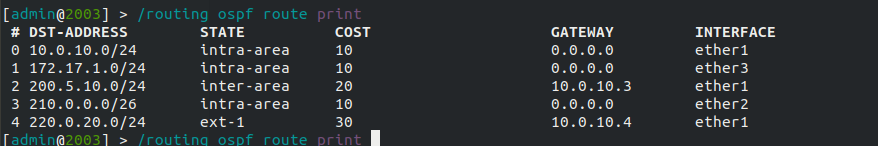
\includegraphics[width=0.7\columnwidth]{figure/routes_stub_area10.png}
			\caption{
					\label{fig:samplesetup} % spaces are big no-no 
					Rutas aprendidas en router 2003 después de definir el área como \textit{stub}.
			}
		\end{figure}
		
		\item \textbf{Capturar tráfico en el área backbone. Deshabilitar y habilitar la interface ether2 de 2007, ¿cómo se publican las redes del entorno RIP? ¿Existe algún LSA de tipo 5? ¿Por qué existe?}\\
		Los cambios en las redes se publican a través de un mensaje LS Update donde se encuentran los LSA de tipo 1 y 5. El primero advierte un cambio en la interfaz del router y el segundo advierte un resumen de las rutas aprendidas externamente.

		\begin{figure}[H] 
			
			\centering 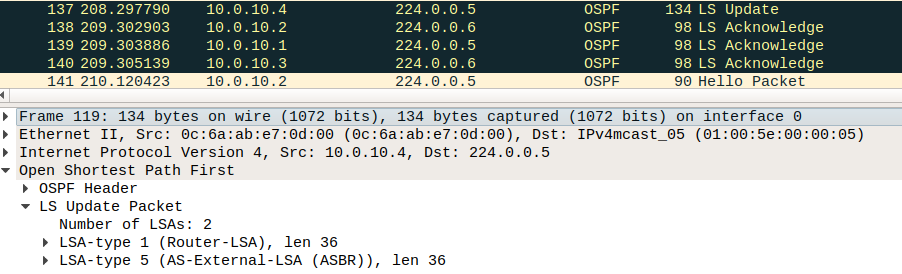
\includegraphics[width=0.7\columnwidth]{figure/ls_update.png}
			\caption{
					\label{fig:samplesetup} % spaces are big no-no 
					Mensajes capturados en la interfaz ether1 en el router 2007 después de habilitar/deshabilitar la interfaz ether2.
			}
		\end{figure}
	\end{enumerate}

	\subsection{Enlaces consultados}
		\begin{itemize}
			\item{HCNA Networking Study Guide}  \\
			\textit{Springer. Huawei Technologies Co., Ltd.},Ch 8.2 RIP.
			\item \href{https://www.juniper.net/documentation/en_US/junos/topics/concept/ospf-stub-áreas-overview.html}
			{Understanding OSPF Stub Areas, Totally Stubby Areas, and Not-So-Stubby Areas}
			\item \href{https://www.juniper.net/documentation/en_US/junos/topics/concept/ospf-routing-external-metrics-overview.html} 
			{Understanding OSPF External Metrics}
			\item \href{https://wiki.mikrotik.com/wiki/Manual:Routing/OSPF}
			{Manual:Routing/OSPF}

		\end{itemize}
\end{document}